\documentclass[mathserif]{beamer}

\setbeamertemplate{frametitle}[default][center]%Centers the frame title.
\setbeamertemplate{navigation symbols}{}%Removes navigation symbols.
\setbeamertemplate{footline}{\raisebox{5pt}{\makebox[\paperwidth]{\hfill\makebox[10pt]{\scriptsize\insertframenumber}}}}

\usepackage{amsmath,amssymb,amsthm}
\usepackage{graphicx,array,dsfont}
\usepackage{harvard}
\citationmode{abbr}

\newcommand{\Hrule}{\rule{\linewidth}{0.2pt}}
\newcommand{\argmax}{\mathop{\mathrm{argmax}}}
\newcommand{\argmin}{\mathop{\mathrm{argmin}}}
\newcommand{\minimize}{\mathop{\mathrm{minimize}}}
\def\half{\frac{1}{2}}
\def\th{\mathrm{th}}
\def\sign{\mathrm{sign}}
\def\supp{\mathrm{supp}}
\def\E{\mathrm{E}}
\def\P{\mathrm{P}}
\def\Var{\mathrm{Var}}
\def\Cov{\mathrm{Cov}}
\def\R{\mathds{R}} 
\def\cA{\mathcal{A}}
\def\cB{\mathcal{B}}
\def\cE{\mathcal{E}}
\def\cF{\mathcal{F}}
\def\cG{\mathcal{G}}
\def\cN{\mathcal{N}}
\def\red{\color[rgb]{0.8,0,0}}
\def\white{\color[rgb]{1,1,1}}
\def\blue{\color[rgb]{0,0,0.8}}

\begin{document}

\title{k-means continued}
\author{Rebecca C. Steorts}
\begin{frame}
\titlepage
{\it Optional reading: ISL 10.3, ESL 14.3}
\end{frame}

\begin{frame}
\frametitle{Announcements}
\begin{enumerate}
\item Monday: Special Lecture at \url{https://duke.zoom.us/j/3768448585} by Brian Kundinger at 11:30 AM.
\item Wednesday live lecture.
\item Friday: office hours with Athena in Old Chem 116. 
\end{enumerate}
\vspace*{1em}
Please read this paper for Monday's presentation \url{https://imai.fas.harvard.edu/research/files/linkage.pdf} and note the connection with mixture models and the EM algorithm. 

\vspace*{1em}
What is Brian presenting: Two novel extensions of Bayesian mixture models. One scales quadratically with the data and the other scales linearly. The application is entity resolution with applications to human rights, voter registration data, medical, among others.
\end{frame}

\begin{frame}
\frametitle{Announcements}
\begin{enumerate}
\item Exam 2: Released Monday, November 18. Due Monday, November 25.
\item Exam 3: Released Monday, December 2. Due Friday, December 6. 
\end{enumerate}

\vspace*{1em}
Will discuss content and exam structure closer to the exams.


\end{frame}

\begin{frame}
\frametitle{Dissimilarity and within-cluster scatter}

Assume observations $X_1,\ldots X_n$, and 
{\blue dissimilarites} $d(X_i,X_j)$.
\bigskip

%Example: $X_i$ is vector $\in \R^p$ and $d(X_i,X_j)=\|X_i-X_j\|_2^2$.\footnote{This is the squared Euclidean distance.}
%\bigskip

Let $K$ be the {\blue number of clusters} (fixed).
\bigskip

A {\blue clustering} of data points
$X_1,\ldots X_n$ is a function $C$ that
assigns each observation $X_i$ to a group (or cluster) $k \in \{1,\ldots K\}$
\end{frame}

\begin{frame}
\frametitle{Dissimilarity and within-cluster scatter}


Let $C(i)=k$ denote
that $X_i$ is assigned to group (or cluster) $k$. 

Let $n_k$ be the number of data points in the group (or cluster) $k$. 
 
Let $d_{ij}=d(X_i,X_j).$

\pause
\bigskip
The {\blue within-cluster scatter} is defined as 
$$W = \half \sum_{k=1}^K 
\frac{1}{n_k} \sum_{C(i)=k, \, C(j)=k} d_{ij}$$

\bigskip
Smaller $W$ is better
\end{frame}

\begin{frame}
\frametitle{Simple example}
\begin{tabular}{cc}
\parbox{0.5\textwidth}{
\centering
Here $n=5$ and $K=2$,\\
$X_i \in \R^2$ and
$d_{ij}=\|X_i-X_j\|_2^2$

\bigskip
{\footnotesize
\begin{tabular}{|c|c|c|c|c|c|}
\hline
& 1 & 2 & 3 & 4 & 5 \\
\hline
1 & 0 & 0.25 & 0.98 & 0.52 & 1.09 \\
\hline
2 & 0.25 & 0 & 1.09 & 0.53 & 0.72 \\
\hline
3 & 0.98 & 1.09 & 0 & 0.10 & 0.25 \\
\hline
4 & 0.52 & 0.53 & 0.10 & 0 & 0.17 \\
\hline
5 & 1.09 & 0.72 & 0.25 & 0.17 & 0 \\
\hline
\end{tabular}}
} \hspace{5pt} & 
\parbox{0.5\textwidth}{
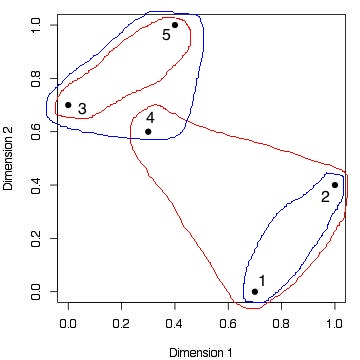
\includegraphics[width=0.4\textwidth]{figures/simple2.jpg}}
\end{tabular}
\begin{itemize}

\bigskip
\item {\red Red clustering}:
$W_{\text{red}}=(0.25+0.53+0.52)/3 + 0.25/2 = 0.56$
\item {\blue Blue clustering}:
$W_{\text{blue}}=0.25/2 + (0.10+0.17+0.25)/3 = 0.30$
\end{itemize}

\bigskip
(Tip: {\tt dist} function in R)
\end{frame}

\begin{frame}
\frametitle{Finding the best group assignments}
Smaller $W$ is better, so why don't we just directly
find the clustering $C$ that {\blue minimizes $W$}?

\bigskip
Problem: doing so requires trying 
{\blue all possible assignments} of the $n$ points into
$K$ groups. The number of possible assignments is
\vspace{-5pt}
$$A(n,K) = \frac{1}{K!}\sum_{k=1}^K (-1)^{K-k} 
{K \choose k} k^n
\vspace{-5pt}$$
Note that $A(10,4)=34,105$, and
$A(25,4) \approx 5 \times 10^{13}$ ... huge
% Jain and Dubes (1998), ``Algorithms for Clustering Data''

\bigskip
Most problems we look at are going to have way 
more than $n=25$ observations, and potentially more
than $K=4$ clusters too! 

\bigskip
So we'll have to settle for an {\blue approximation}
\end{frame}

\begin{frame}
\frametitle{Rewriting the within-cluster scatter}
Focus on Euclidean space: now $X_i \in \R^p$ and
dissimilarities are $d(X_i,X_j)=\|X_i-X_j\|_2^2$

\bigskip
Fact: within-cluster scatter can
be rewritten as
$$\half\sum_{k=1}^K \frac{1}{n_k} \sum_{C(i)=k} 
\sum_{C(j)=k} \|X_i-X_j\|_2^2 = 
\sum_{k=1}^K \sum_{C(i)=k} \|X_i-\bar{X}_k\|_2^2$$
with $\bar{X}_k$ the average of points
in group $k$,  
$\bar{X}_k = \frac{1}{n_k} \sum_{C(i)=k} X_i$.
The right-hand side above is called
{\blue within-cluster variation}

\bigskip
Hence, equivalently we seek 
a clustering $C$ that minimizes
the within-cluster variation (approximately so)
\end{frame}

\begin{frame}
\frametitle{Rewriting the minimization}
Remember: we want to choose $C$ to minimize
\vspace{-5pt}
$$\sum_{k=1}^K \sum_{C(i)=k} \|X_i-\bar{X}_k\|_2^2
\vspace{-5pt}$$

\bigskip
Another fact: for any $Z_1,\ldots Z_m \in \R^p$, the 
quantity $\sum_{i=1}^m \|Z_i-c\|_2^2$ is minimized by 
taking 
$c=\bar{Z}=\frac{1}{m} \sum_{i=1}^m Z_i$, the average
of the $Z_i$'s

\bigskip
So our problem is the same as minimizing the 
{\blue enlarged criterion}
\vspace{-5pt}
$$\sum_{k=1}^K \sum_{C(i)=k} \|X_i-c_k\|_2^2,
\vspace{-5pt}$$
over both clusterings $C$ and $c_1,\ldots c_K\in\R^p$
\end{frame}

\begin{frame}
\frametitle{$K$-means algorithm}

\begin{enumerate}
\item Cluster (label) each point based the closest 
center
\item Replace each center by the average of points in 
its cluster
\end{enumerate}
\vspace*{1em}
\end{frame}


\begin{frame}
\frametitle{$K$-means algorithm}
The {\blue $K$-means} clustering algorithm approximately 
minimizes the enlarged criterion 
by {\blue alternately minimizing} over $C$ and 
$c_1,\ldots c_K$

\bigskip
We start with an initial guess for $c_1,\ldots c_K$
(e.g., pick $K$ points at random over the range of
$X_1,\ldots X_n$), then repeat:
\begin{enumerate}
\item {\blue Minimize over $C$}: for each  
$i=1,\ldots n$, find the cluster center $c_k$ closest 
to $X_i$, and let $C(i)=k$
\item {\blue Minimize over $c_1,\ldots c_K$}: for each 
$k=1,\ldots K$, let $c_k = \bar{X}_k$,
the average of points in group $k$
\end{enumerate}
Stop when within-cluster variation doesn't change


\end{frame}

\begin{frame}
\frametitle{$K$-means example}
\smallskip
\smallskip
Here $X_i \in \R^2$, $n=300$, and $K=3$

\begin{center}
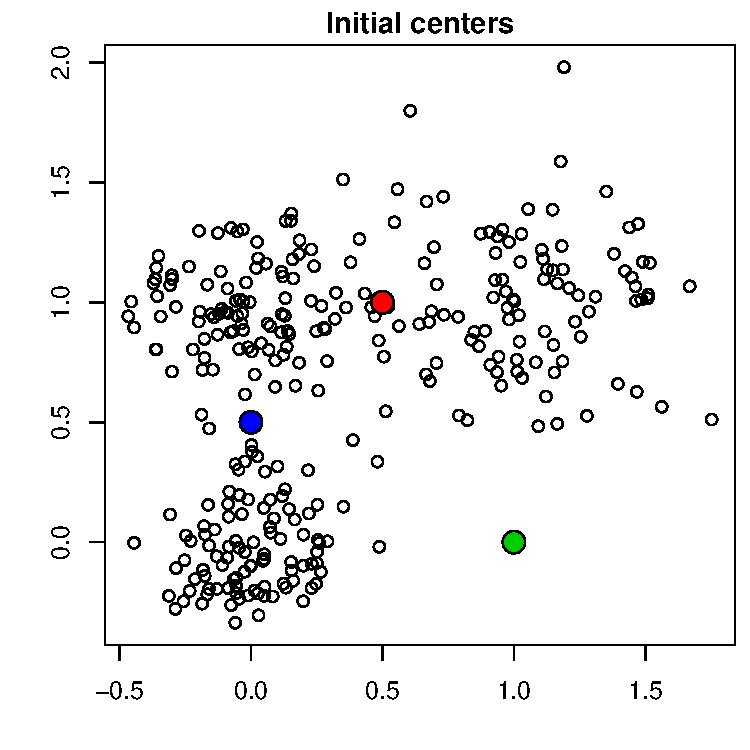
\includegraphics[width=0.31\textwidth]{km0.pdf}
\hspace{3pt}
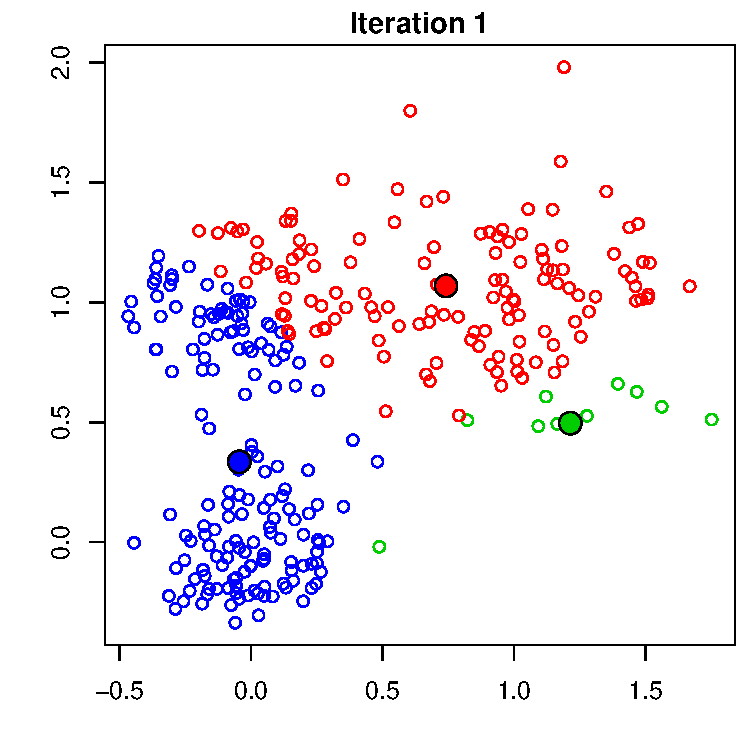
\includegraphics[width=0.31\textwidth]{km1.pdf} 
\hspace{3pt}
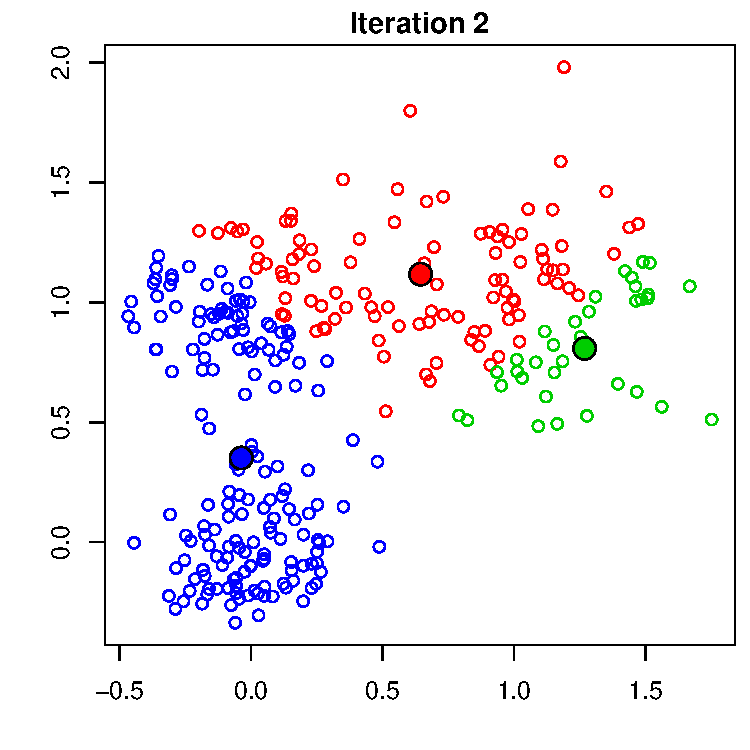
\includegraphics[width=0.31\textwidth]{km2.pdf} \\
\smallskip
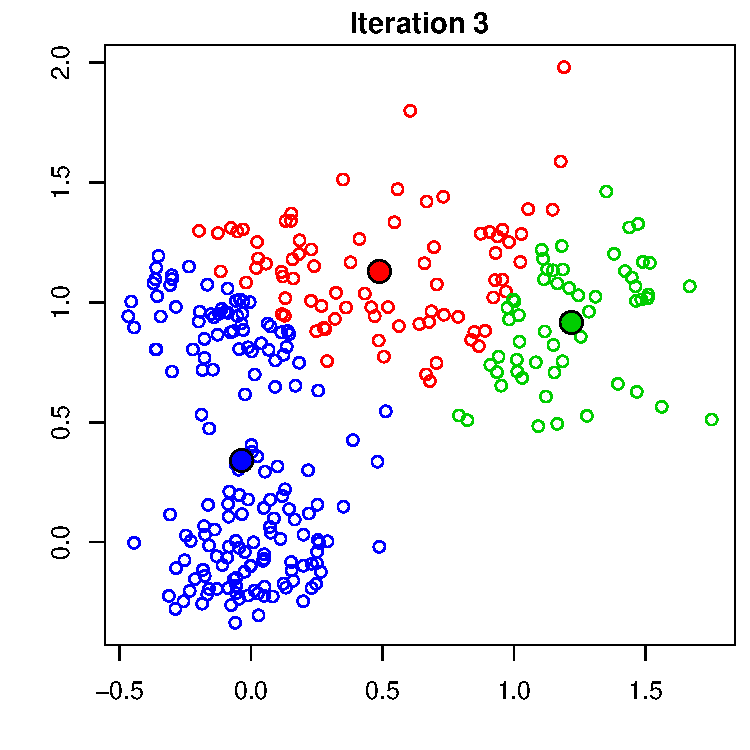
\includegraphics[width=0.31\textwidth]{km3.pdf} 
\hspace{3pt}
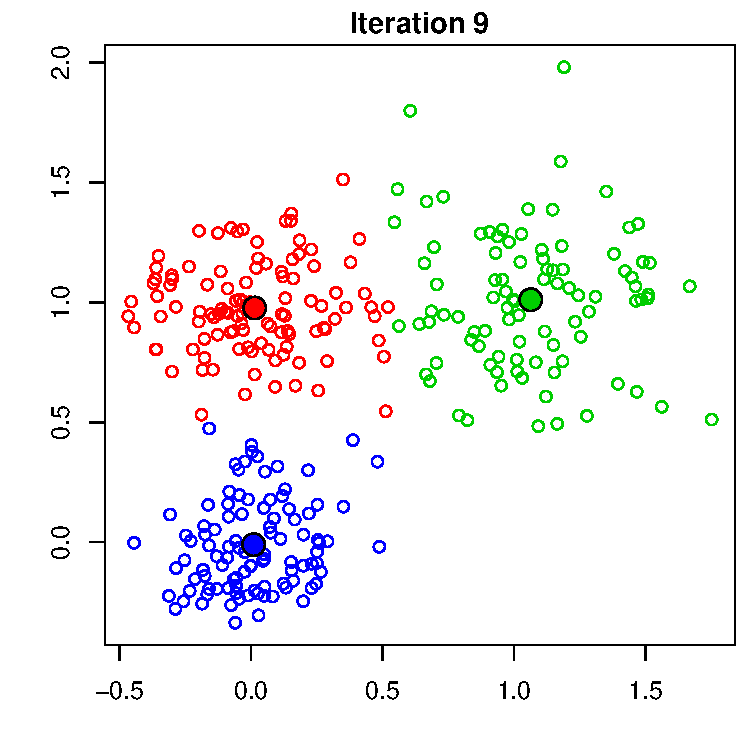
\includegraphics[width=0.31\textwidth]{km9.pdf} 
\end{center}
\end{frame}

%\begin{frame}
%\frametitle{Voronoi tessellation}
%
%\begin{tabular}{cc}
%\parbox{0.5\textwidth}{
%Given cluster centers, we identify each point to 
%its nearest center. This defines a
%{\red Voronoi tessellation} of $\R^p$} &
%\hspace{-15pt}
%\parbox{0.5\textwidth}{
%\includegraphics[width=0.5\textwidth]{vor.pdf}}
%\end{tabular}
%
%\vspace{-5pt}
%Given $c_1,\ldots c_K \in \R^p$, we define 
%the Voronoi sets
%$$V_k = \{x \in \R^p: 
%\|x-c_k\|_2^2 \leq \|x-c_j\|_2^2, \, j=1,\ldots K\},
%\;\,k=1,\ldots K$$
%These are {\red convex polyhedra} (we'll see them
%again when we study classification)
%\end{frame}

\begin{frame}
\frametitle{Properties of $K$-means}
\begin{itemize}
\item Within-cluster variation {\blue decreases}
with each iteration of the algorithm. I.e., if $W_t$ 
is the within-cluster variation at iteration $t$, 
then $W_{t+1} \leq W_t$ 
\item The algorithm {\blue always converges}, no
matter the initial cluster centers. In fact, it takes
$\leq K^n$ iterations (why?)
\item The final clustering {\blue depends on the initial}
cluster centers. Sometimes, different initial centers
lead to very different final outputs. 
So we typically run $K$-means {\blue multiple times} 
(e.g., 10 times),
randomly initializing cluster centers for each run,
then choose among from collection of centers 
based on which one gives the smallest 
within-cluster variation
\item The algorithm is {\blue not guaranteed} to deliver
the clustering that globally minimizes
within-cluster variation (recall: this would require  
looking through all possible assignments!)
\end{itemize}
\end{frame}

\begin{frame}
\frametitle{$K$-means example, multiple runs}
Here $X_i \in \R^2$, $n=250$, and $K=4$,
the points are not as well-separated

\bigskip
\begin{tabular}{ccc}
\hspace{-26pt} 
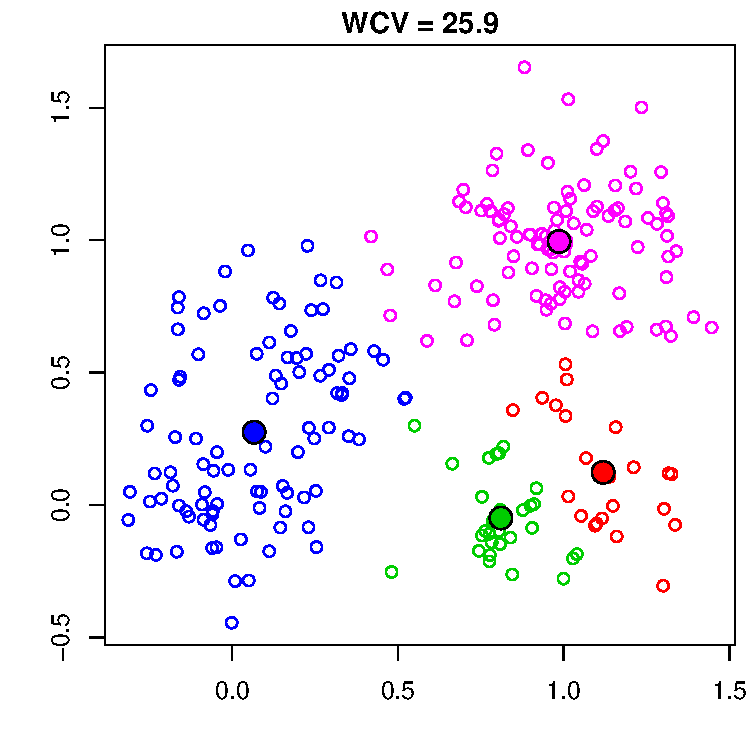
\includegraphics[width=0.36\textwidth]{figures/kmm1.pdf} &
\hspace{-17pt}
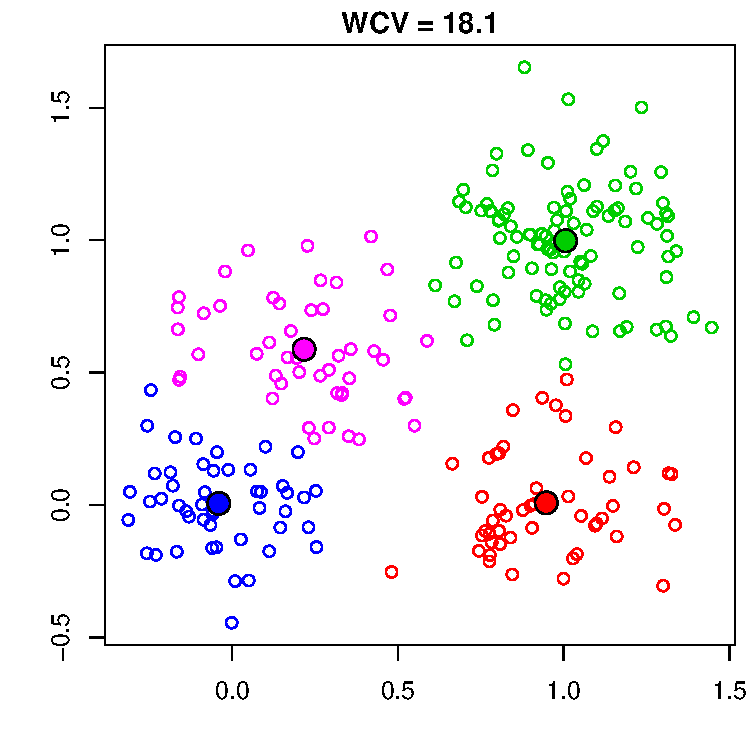
\includegraphics[width=0.36\textwidth]{figures/kmm2.pdf} &
\hspace{-17pt}
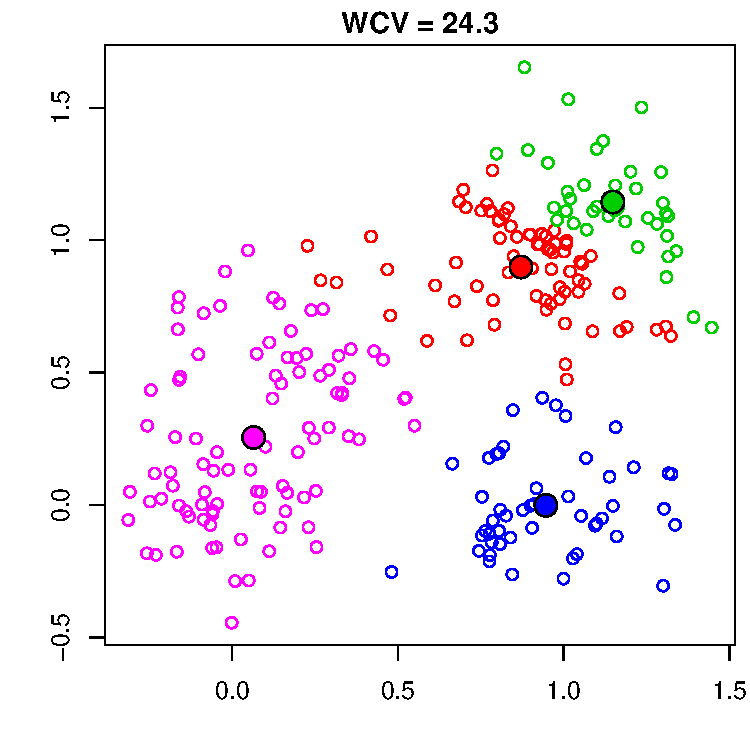
\includegraphics[width=0.36\textwidth]{figures/kmm3.pdf}
\end{tabular}

\smallskip
These are results of result of running the $K$-means
algorithm with different initial centers (chosen randomly
over the range of the $X_i$'s). We choose the second
collection of centers because it yields the 
{\blue smallest within-cluster variation}
\end{frame}

%\begin{frame}
%\frametitle{Vector quantization}
%(Example from ESL p. 514.) Left: original image;
%middle: using 23.9\% of the storage; right: using 6.25\% of 
%the storage
%
%\smallskip
%\includegraphics[width=\textwidth]{vq.pdf} 
%
%\smallskip
%\smallskip
%$K$-means is often called ``Lloyd's algorithm'' in computer 
%science and engineering, and is used in {\red vector 
%quantization} for compression
%
%\bigskip 
%Basic idea: run $K$-means clustering on $4\times 4$ squares 
%of pixels in an image, and keep only the clusters and labels.
%Smaller $K$ means more compression
%\end{frame}

\begin{frame}
\frametitle{In $K$-means, cluster centers are averages}
\smallskip
A cluster center is representative for all 
points in a cluster, also called a 
{\blue prototype}

\bigskip
In $K$-means, we simply take a cluster center to be 
the {\blue average} of points in the cluster.
Great for computational purposes---but how
does it lend to {\blue interpretation}?

\bigskip
This would be fine if we were clustering, e.g., houses in 
Durham based on features like price, square footage,
number of bedrooms, distance to nearest bus stop, etc.

\bigskip
We have to be careful as some applications may not be well suited to k-means. For instance, 
any applications where the data overlaps would not work well. Examples: entity resolution, network analysis, medical data, and others.

%\bigskip
%Not so if we were clustering faces
%of statistics professors (why?)
%
%\vspace{-5pt}
%\begin{center}
%\includegraphics[height=0.9in]{tibs.jpg}
%\hspace{2pt}
%\includegraphics[height=0.9in]{shalizi.jpg}
%\hspace{2pt}
%\includegraphics[height=0.9in]{nugent.jpg}
%\hspace{2pt}
%\includegraphics[height=0.9in]{greenhouse.jpg}
%\hspace{2pt}
%\includegraphics[height=0.9in]{junker.jpg}
%\end{center}
\end{frame}

\begin{frame}
\smallskip
\frametitle{$K$-medoids algorithm}
In some applications we want each center
to be {\blue one of the points} itself.
This is where {\blue $K$-medoids} comes in---an
algorithm similar to 
the $K$-means algorithm, except when fitting
the centers $c_1,\ldots c_K$, we restrict our
attention to the points themselves

\bigskip
Initial guess for centers $c_1,\ldots c_K$ (e.g., randomly
select $K$ of the points $X_1,\ldots X_n$), then repeat:
\begin{enumerate}
\item {\blue Minimize over $C$}: for each  
$i=1,\ldots n$, find the cluster center $c_k$ closest 
to $X_i$, and let $C(i)=k$
\item {\blue Minimize over $c_1,\ldots c_K$}: for each 
$k=1,\ldots K$, let $c_k = X^*_k$, the
{\blue medoid} of points in cluster $k$, i.e., the point 
$X_i$ in cluster $k$ that minimizes
$\sum_{C(j)=k} \|X_j-X_i\|_2^2$
\end{enumerate}
Stop when within-cluster variation doesn't change

\bigskip
In words:
\begin{enumerate}
\item Cluster (label) each point based on the closest center
\item Replace each center by the medoid of points in its cluster
\end{enumerate}
\end{frame}

\begin{frame}
\frametitle{$K$-medoids example}
\begin{center}
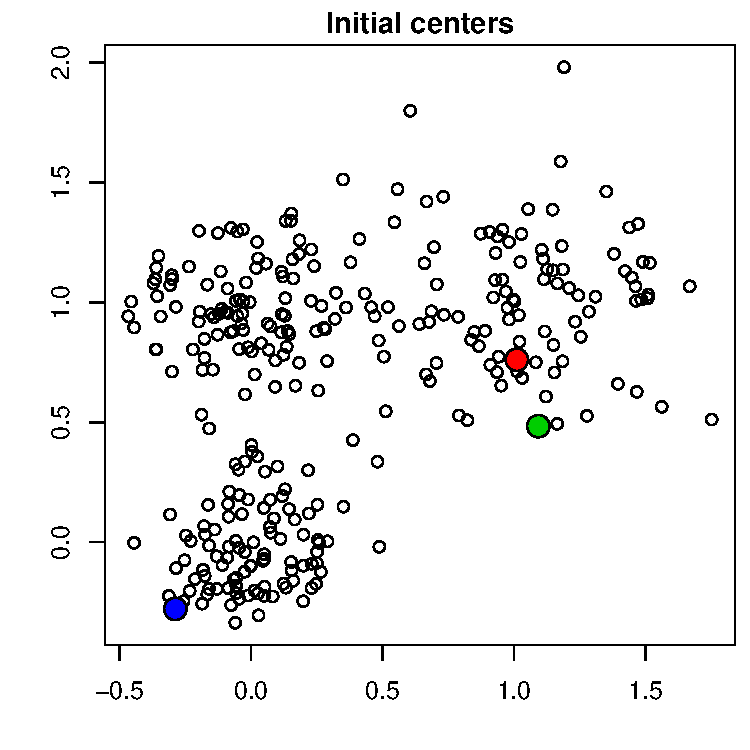
\includegraphics[width=0.31\textwidth]{figures/kmed0.pdf}
\hspace{3pt}
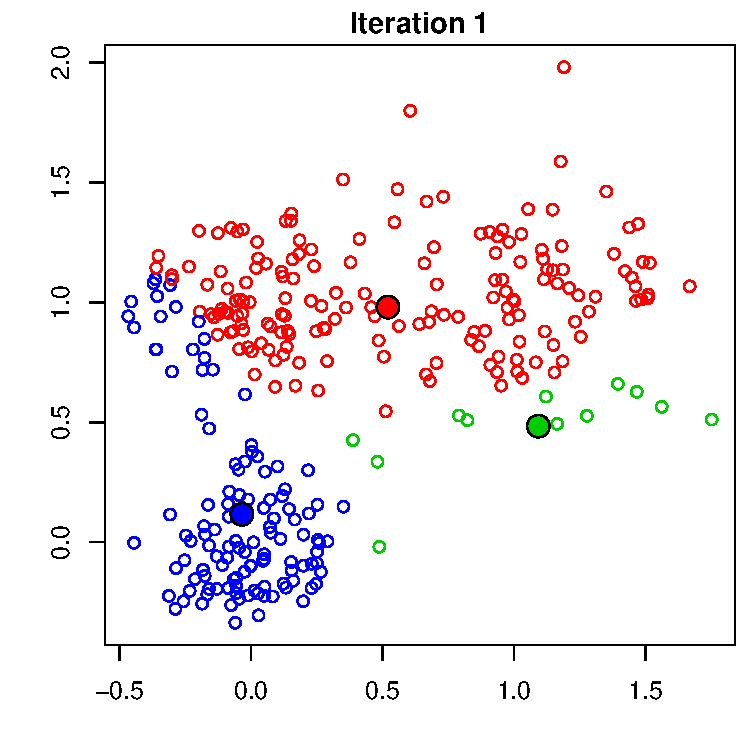
\includegraphics[width=0.31\textwidth]{figures/kmed1.pdf} 
\hspace{3pt}
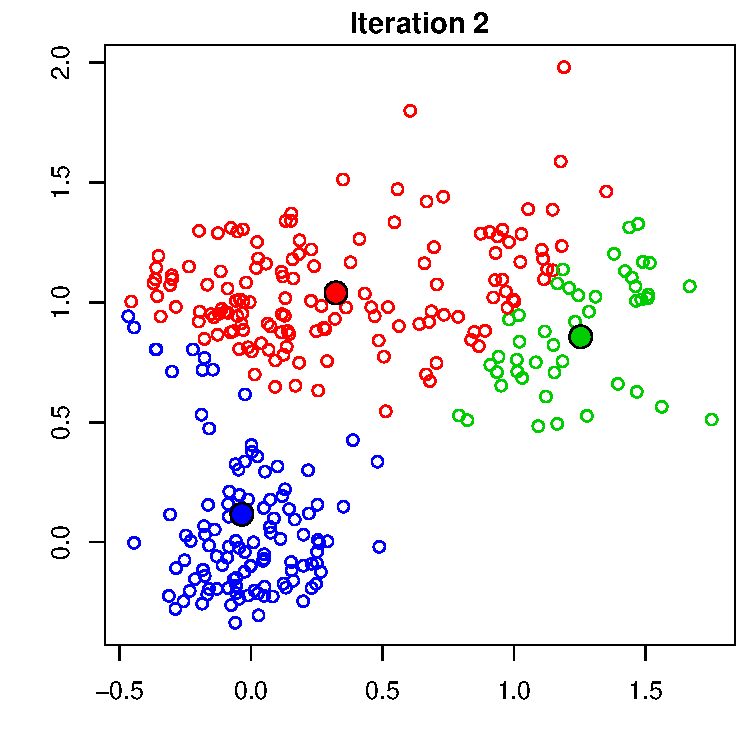
\includegraphics[width=0.31\textwidth]{figures/kmed2.pdf} \\
\smallskip
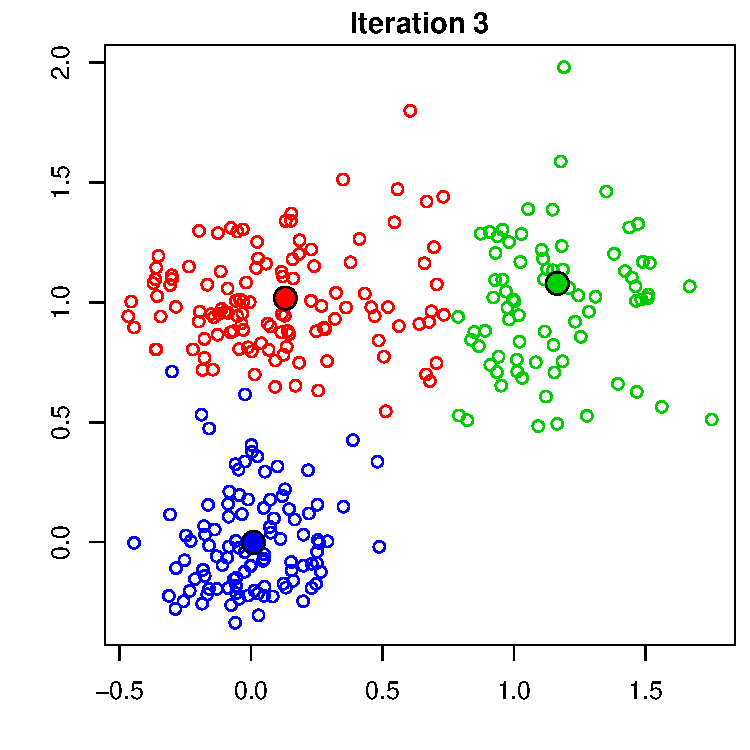
\includegraphics[width=0.31\textwidth]{figures/kmed3.pdf} 
\hspace{3pt}
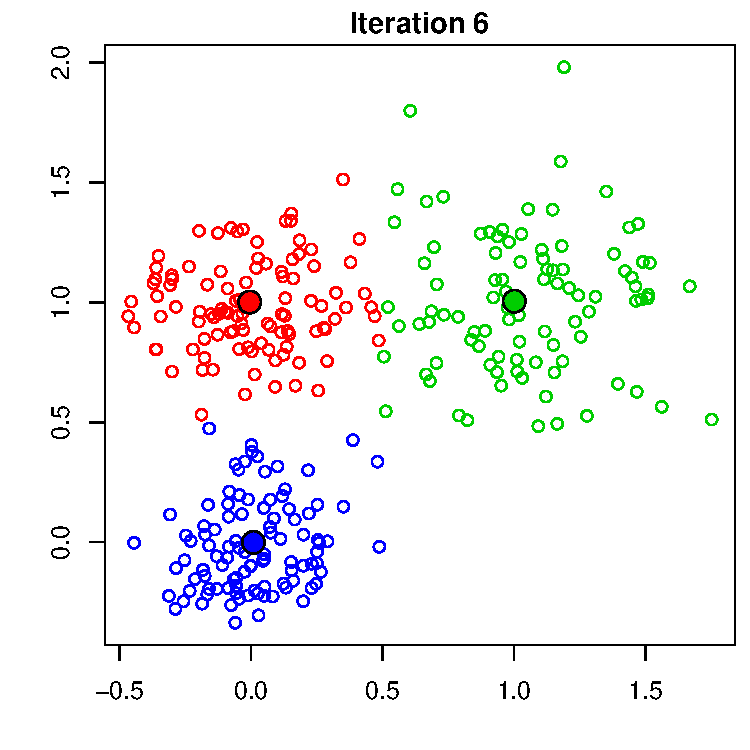
\includegraphics[width=0.31\textwidth]{figures/kmed6.pdf} 
\end{center}

\smallskip
Note: only 3 points had different labels under $K$-means
\end{frame}

\begin{frame}
\frametitle{Properties of $K$-medoids}
The $K$-medoids algorithm 
{\blue shares the properties}
of $K$-means that we discussed (each iteration 
decreases the criterion; the algorithm
always converges; different starts gives
different final answers; it does 
not achieve the global minimum)

\bigskip
$K$-medoids generally returns
a {\blue higher value} of 
$$\sum_{k=1}^K \sum_{C(i)=k} \|X_i-c_k\|_2^2$$
than does $K$-means (why?).
Also, $K$-medoids is {\blue computationally
harder} than $K$-means (because of step 
2: computing the medoid is harder than
computing the average)

\bigskip
Remember, $K$-medoids has the (potentially 
important) property that the centers are located among
the data points themselves
\end{frame}

\begin{frame}[fragile]
\frametitle{$K$-means and $K$-medoids in R}
The $K$-means algorithm is part of the base 
distribution in R, given by the {\tt kmeans} function 
(use {\tt algorithm="Lloyd"})

\bigskip
E.g.,
\begin{verbatim}
km = kmeans(x, centers=k, nstart=10, algorithm="Lloyd")
\end{verbatim}

\bigskip
The $K$-medoids algorithm is implemented by the
function {\tt pam} (stands ``for partitioning
around medoids'') in the package {\tt cluster}
\end{frame}

\begin{frame}
\frametitle{Recap: clustering}
In {\blue clustering} we divide up our data points
into groups or clusters. We want points
in any one group to be more similar to each other
than to other points. All based on pairwise
dissimilarities $d_{ij}$

\bigskip
Fixing the number of clusters $K$, the task of 
exactly minimizing the 
{\blue within-cluster
variation} (equivalently, 
{\blue within-cluster scatter})
is not feasible. The {\blue $K$-means algorithm} 
approximately minimizes this by iterating two
simple steps

\bigskip
Though it always converges, the answer given
by $K$-means depends on the initial centers. It 
also returns centers that are averages of data
points. The {\blue $K$-medoids algorithm} is an
alternative where the centers are chosen among 
the points themselves. Its answer also depends on the 
starting configuration.
Hence for either algorithm, one should {\blue run it
several times} with different starts
\end{frame}






\end{document}
